\subsection{Algorithm}

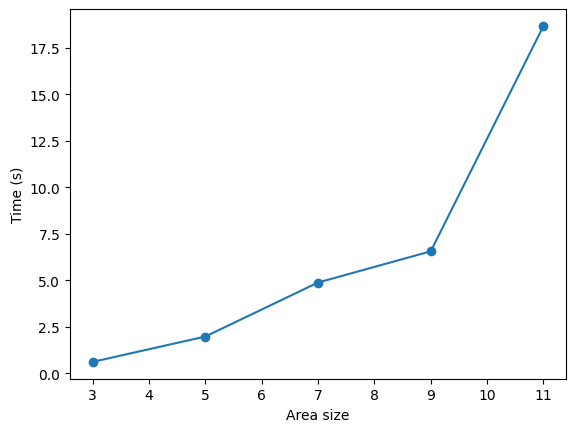
\includegraphics[scale=0.5]{images/time_area.png}

As shown, the computation time increases exponentially with area.
Alternatives are - bidirectional RRT and D star.
What could be improved / is it practical? TODO
 
\subsection{Global planner}

The global planner provides a series goals for every drone in the global frame, scouting the entire region. This is done by converting the grid into polar coordinates and equally distributing regions for each drone to visit. This is indeed practical and faster compared to an alternative approach where the planning is done in Cartesian coordinates, shown by the x percent reduction in compute time. TODO

In practice, the global planner could use a satellite image of a forest and plan drones to cover it. 

Complexity
What could be improved / is it practical?
Alternatives
Supported by results

\subsection{Local maps}

To reduce overall computation time, RRT computes multiple obstacle free paths
using a series of local maps to reach the global goal [refer results]. This is done by slicing sections of the global occupancy map just enough to include the next goal given by the global planner to avoid use of a global occupancy map. By doing this the computation time is reduced by x. TODO \\ 

\subsection{Obstacle detections}
With that said, all obstacles are revealed within a local map for the drone to compute a obstacle free path. The local map's dimensions can differ depending on the global map and grid size, which means detecting all obstacles within a local map is unlikely in the real world where sensors have a limited range of detection. \\
 A potential improvement here to imitate a real world scenario is using a dynamic local map and revealing obstacles only within a certain radius of the drone.

